\documentclass[conference]{IEEEtran}

% ─── Packages ─────────────────────────────────────────────
\usepackage{cite}
\usepackage{amsmath,amssymb,amsfonts}
\usepackage{algorithmic}
\usepackage{algorithm}
\usepackage{graphicx}
\usepackage{textcomp}
\usepackage{xcolor}
\usepackage{booktabs}
\usepackage{url}
\usepackage{hyperref}
\usepackage{balance}
\usepackage{subcaption}
\usepackage{listings}
\usepackage{tikz}
\usetikzlibrary{arrows.meta, positioning, shapes.geometric, fit, backgrounds, calc}

% ─── Draft helpers (remove for final) ─────────────────────
% \newcommand{\todo}[1]{\textcolor{red}{\textbf{[TODO: #1]}}}
\newcommand{\rqone}{\textbf{RQ1}}
\newcommand{\rqtwo}{\textbf{RQ2}}
\newcommand{\rqthree}{\textbf{RQ3}}

\begin{document}

\title{Cross-Level Risk Propagation: Bridging Method-Level\\Architecture with Ecosystem-Level Dependency Analysis}

\author{
    \IEEEauthorblockN{Anonymous Author}
    \IEEEauthorblockA{
        \textit{Master of Computer Information Systems}\\
        \textit{University}\\
        email@university.edu
    }
    \and
    \IEEEauthorblockN{Anonymous Co-Author}
    \IEEEauthorblockA{
        \textit{Department of Computer Science}\\
        \textit{University}\\
        collaborator@university.edu
    }
}

\maketitle

% ══════════════════════════════════════════════════════════════
% §0 ABSTRACT
% ══════════════════════════════════════════════════════════════
\begin{abstract}
Modern software supply chains introduce risk at two distinct granularities: the \emph{ecosystem level}, where packages form massive dependency graphs, and the \emph{method level}, where individual functions carry architectural complexity.
Existing Software Composition Analysis (SCA) tools operate at a single level—either flagging vulnerable packages without inspecting their internals, or analyzing code structure without considering ecosystem context.
We present \textsc{Oscar}, a framework that bridges these levels through a novel \emph{cross-level risk propagation} formula.
Given a root package, \textsc{Oscar} resolves its transitive dependency graph, performs static call-graph construction on each critical dependency, and computes a unified risk score that combines method-level composite risk with ecosystem-wide fan-in.
We evaluate \textsc{Oscar} on a corpus of 50 packages across npm and PyPI, demonstrating that cross-level analysis doubles the precision of ecosystem-only vulnerability prioritization (P@5=0.44 vs.\ 0.20), that automated patch mining can recover function-level CVE data for 69\% of advisories where upstream databases provide none, and that the formula produces remarkably stable rankings across four parameterizations (Spearman $\rho \geq 0.97$).
\end{abstract}

\begin{IEEEkeywords}
software supply chain, dependency analysis, call graph, risk propagation, software composition analysis
\end{IEEEkeywords}

% ══════════════════════════════════════════════════════════════
% §1 INTRODUCTION
% ══════════════════════════════════════════════════════════════
\section{Introduction}
\label{sec:introduction}

Modern software systems are predominantly assembled from open-source components. Recent industry surveys report that 80--97\% of codebases contain open-source dependencies~\cite{synopsys2024}, with a typical application transitively depending on hundreds or thousands of packages. This dependency model delivers enormous productivity gains but introduces a fundamental risk management challenge: how should developers prioritize security and maintenance effort across a supply chain they neither control nor fully understand?

The dominant approach today is \emph{Software Composition Analysis} (SCA). Tools such as Snyk~\cite{snyk2024}, Dependabot~\cite{dependabot}, and Google's OSV~\cite{osv} monitor dependency graphs for known vulnerabilities (CVEs) and alert developers when an affected package version appears in their transitive closure. While effective at detection, these tools operate at a single level of abstraction---the \emph{package level}---treating each dependency as an opaque unit. This produces two systematic failure modes:

\textbf{False positives from unreachable code.} A CVE in a transitive dependency may target a function that is \emph{never reachable} from the root package's public API. Without inspecting the internal structure of the affected package, SCA tools cannot distinguish exploitable vulnerabilities from dead code. Prior work has shown that up to 73\% of flagged CVEs may be unreachable in practice~\cite{pashchenko2020vuln4real}.

\textbf{Blind spots from hidden amplifiers.} Conversely, package-level metrics miss \emph{micro-dependencies}---tiny packages with minimal code but massive ecosystem fan-in. Our analysis reveals that \texttt{ms}, a single-file time conversion utility in npm, is transitively depended upon by over 828,000 packages. A structurally complex method inside such a package carries risk far exceeding its internal metrics alone, yet no SCA tool surfaces this cross-level relationship.

The root cause of both failures is the \emph{level separation}: ecosystem-level tools ignore method-level architecture, while code-quality tools (SonarQube, CodeClimate) ignore ecosystem context. No existing framework bridges these levels to produce a unified risk assessment.

\textbf{This paper.} We propose \emph{cross-level risk propagation}, a formula that combines method-level architectural risk (complexity, centrality, blast radius, code churn) with ecosystem-level structural importance (global fan-in). We implement this approach in \textsc{Oscar}, a multi-tier framework consisting of a Dependency Observatory, a Method Observatory, and a cross-level orchestrator. Given a root package, \textsc{Oscar} resolves its full transitive dependency graph, performs static call-graph construction on each structurally critical dependency, and returns a unified ranking of the riskiest methods across the entire supply chain.

Our contributions are:
\begin{enumerate}
    \item A \textbf{cross-level risk formula} that bridges method-level composite risk with ecosystem fan-in through logarithmic dampening, along with a formal \emph{internal resolution rate} metric that serves as a confidence gate for call-graph quality (§\ref{sec:approach}).
    \item The \textbf{\textsc{Oscar} framework}: an open-source, multi-tier platform implementing cross-level analysis across npm and PyPI with on-demand ingestion, static call-graph construction, and intra-dependency reachability filtering (§\ref{sec:framework}).
    \item An \textbf{empirical evaluation} on 50 packages across two ecosystems, demonstrating that cross-level analysis surfaces high-risk methods invisible to single-level tools, provides stable rankings across formula variants ($\rho \geq 0.97$), and identifies 12 ``hidden amplifier'' micro-dependencies with outsized supply chain risk (§\ref{sec:evaluation}).
\end{enumerate}

% ══════════════════════════════════════════════════════════════
% §2 RELATED WORK
% ══════════════════════════════════════════════════════════════
\section{Related Work}
\label{sec:related}

Our work sits at the intersection of four active research areas. We survey each and position our contribution relative to the state of the art.

\subsection{Software Composition Analysis}

SCA tools identify known vulnerabilities in open-source dependencies by matching package versions against advisory databases. Commercial tools such as Snyk~\cite{snyk2024} and GitHub's Dependabot~\cite{dependabot} automate this matching, while open databases like OSV~\cite{osv} and the National Vulnerability Database provide machine-readable advisory feeds. OWASP Dependency-Check performs similar matching for Java, .NET, and Python ecosystems.

A fundamental limitation of all current SCA tools is that they operate at the \emph{package level}: a CVE is either ``in your dependencies'' or not. No mainstream SCA tool inspects the internal method-level structure of affected packages to assess whether the vulnerable code is actually reachable. Pashchenko et al.~\cite{pashchenko2020vuln4real} demonstrated that this leads to significant over-reporting, as many flagged vulnerabilities reside in code paths unused by downstream consumers.

\textsc{Oscar} addresses this gap by \emph{combining} package-level dependency analysis with method-level call-graph inspection, enabling reachability-aware vulnerability assessment.

\subsection{Static Call Graph Construction}

Static call-graph construction has been extensively studied for Java (WALA, Soot~\cite{lam2011soot}, Doop~\cite{smaragdakis2015doop}) and more recently for Python (PyCG~\cite{salis2021pycg}). These frameworks construct intra-project call graphs to support program comprehension, refactoring, and security analysis.

PyCG~\cite{salis2021pycg} is the closest prior work for Python. It constructs call graphs by resolving function assignments and class hierarchies, reporting precision of 99.2\% and recall of 69.9\% on a benchmark of small-to-medium Python projects. Critically, PyCG evaluates only \emph{intra-project} edges---calls to external libraries are excluded from its precision/recall measurements. \textsc{Oscar}'s internal resolution rate (§\ref{subsec:resolution-rate}) follows the same methodological boundary, making PyCG's evaluation protocol directly comparable to ours.

A key distinction is that PyCG and similar tools analyze a \emph{single project} in isolation. They produce method-level metrics but have no concept of how those metrics relate to the package's ecosystem-wide importance. \textsc{Oscar} bridges this gap by computing composite risk per method and then scaling it by the package's global fan-in.

Grove and Chambers~\cite{grove2001framework} formalized call graph construction as a family of flow-sensitive algorithms. While their framework is language-agnostic, all practical implementations target a single codebase. Cross-project static analysis remains an open challenge due to the infeasibility of resolving all transitive source code simultaneously.

\subsection{Supply Chain Risk Metrics}

Several metrics have been proposed to quantify supply chain health at the ecosystem level. Cox et al.'s \emph{libyears}~\cite{cox2015measuring} measures dependency freshness as the cumulative time lag between used versions and latest releases. Google's deps.dev~\cite{depsdev} provides pre-computed dependency graphs, version advisories, and license information for major ecosystems. The OpenSSF Scorecard project~\cite{openssf} aggregates security practices (CI/CD, code review, fuzzing) into a per-project health score.

Zimmermann et al.~\cite{zimmermann2019small} conducted the landmark study of the npm ecosystem, identifying both the prevalence of micro-dependencies and the risk of single points of failure in the supply chain graph. Decan et al.~\cite{decan2019empirical} compared seven packaging ecosystems, finding consistent patterns of increasing dependency depths and concentration of maintainership.

All of these metrics operate on \emph{metadata}: version numbers, timestamps, repository activity, or graph topology. None inspects the actual source code of packages to assess \emph{structural} risk at the method level. \textsc{Oscar}'s cross-level formula is the first to combine metadata-based ecosystem importance (fan-in) with source-code-derived method risk (composite risk), producing a score that captures both dimensions.

\subsection{Reachability Analysis for Vulnerability Triage}

The idea of using reachability to filter vulnerability alerts has been explored in both academic and commercial contexts. Eclipse Steady (formerly Vulas)~\cite{plate2015eclipsesteady} performs change-impact analysis on Java applications by computing whether the vulnerable code patch overlaps with code paths reachable from the application's entry points. Ponta et al.~\cite{ponta2018beyond} extended this to a code-centric, usage-based analysis that identifies ``vulnerable constructs'' (the specific functions modified in a fix commit) and checks their reachability via combined static and dynamic analysis. Their approach relies on Project KB~\cite{ponta2019projectkb}, a manually curated dataset mapping CVEs to fix commits. This requires the full application source code and analyzes reachability \emph{from the consumer's perspective}.

Dann et al.~\cite{dann2021identifying} systematically evaluated OSS vulnerability scanners, finding that most lack reachability analysis entirely, and those that include it (Snyk's commercial offering) require language-specific integrations and whole-application context.

\textsc{Oscar} takes a different approach: \emph{intra-dependency reachability}. Rather than requiring the consumer's full source code, \textsc{Oscar} analyzes reachability \emph{within the affected package itself}, asking: ``Is the vulnerable function reachable from this package's own public API?'' This scope is deliberately narrower than whole-application analysis but has a critical practical advantage: it can be computed \emph{for any package on demand}, without access to any specific consumer's codebase. Additionally, where Eclipse Steady relies on manually curated fix-commit mappings, we employ an automated patch mining pipeline that programmatically recovers affected function names from advisory metadata (§\ref{subsec:rq2}). We discuss the trade-offs in §\ref{sec:discussion}.

% ══════════════════════════════════════════════════════════════
% §3 APPROACH
% ══════════════════════════════════════════════════════════════
\section{Approach}
\label{sec:approach}

This section formalizes the cross-level risk propagation model. We first define the individual risk components at each level, then present the formula that bridges them.

\subsection{Threat Model}
\label{subsec:threat-model}

We consider a developer who maintains a \emph{root package} $P_0$ with version $v_0$. The root package transitively depends on packages $P_1, P_2, \ldots, P_k$ through the dependency graph $G_{\mathrm{dep}} = (V, E)$, where $V = \{P_0, P_1, \ldots, P_k\}$ and $(P_i, P_j) \in E$ iff $P_i$ directly depends on $P_j$.

The developer seeks to answer: \emph{``Which individual method, across my entire transitive supply chain, poses the highest combined risk from both architectural complexity and ecosystem-wide exposure?''}

\subsection{Method-Level Composite Risk}
\label{subsec:composite-risk}

For a given package $P_i$, \textsc{Oscar} constructs a static call graph $G_{\mathrm{call}}^{(i)} = (M_i, E_i)$ where $M_i$ is the set of methods (functions, class methods) extracted from the package's source code, and $E_i$ are caller$\to$callee edges.

For each method $m \in M_i$, we compute four structural properties:

\begin{enumerate}
    \item \textbf{Cyclomatic Complexity} $\mathrm{CC}(m)$: the number of linearly independent paths through $m$, computed from control-flow branch points in the AST.
    
    \item \textbf{Centrality} $\mathrm{Cent}(m)$: the normalized degree centrality of $m$ in $G_{\mathrm{call}}^{(i)}$, measuring how many other methods call or are called by $m$:
    \begin{equation}
        \mathrm{Cent}(m) = \frac{\deg_{\mathrm{in}}(m) + \deg_{\mathrm{out}}(m)}{2(|M_i| - 1)}
    \end{equation}
    
    \item \textbf{Blast Radius} $\mathrm{BR}(m)$: the number of methods transitively reachable from $m$ in $G_{\mathrm{call}}^{(i)}$, computed via BFS.
    
    \item \textbf{Temporal Factor} $\mathrm{TF}(m)$: a churn-based amplifier derived from the method's git history. Let $\mathrm{commits}(m)$ be the number of commits modifying the file containing $m$ in the last 6 months, and $\mu_{\mathrm{repo}}$ the repository average. Then:
    \begin{equation}
        \mathrm{TF}(m) = \max\!\left(1.0,\; \frac{\mathrm{commits}(m)}{\mu_{\mathrm{repo}}}\right)
    \end{equation}
    The floor of 1.0 ensures temporal data never \emph{reduces} risk; it only amplifies methods in frequently churned code.
\end{enumerate}

The \textbf{composite risk} of method $m$ is:
\begin{equation}
    \label{eq:composite}
    \mathrm{CompositeRisk}(m) = \mathrm{CC}(m) \times \mathrm{Cent}(m) \times \mathrm{BR}(m) \times \mathrm{TF}(m)
\end{equation}

This score captures the \emph{intra-package} architectural risk: a method that is complex, central to the call graph, has a large blast radius, and is frequently modified carries the highest internal risk.

\subsection{Ecosystem-Level Fan-In}
\label{subsec:fan-in}

At the ecosystem level, we define the \textbf{global fan-in} $\mathrm{FI}(P_i)$ as the number of distinct packages across the entire registry (npm or PyPI) that transitively depend on $P_i$. This quantity is sourced from deps.dev~\cite{depsdev}, which maintains pre-computed dependency graphs for major ecosystems.

Global fan-in captures the \emph{ecosystem exposure}: a vulnerability in a package with $\mathrm{FI} = 800{,}000$ (e.g., \texttt{ms}) affects orders of magnitude more downstream consumers than one with $\mathrm{FI} = 3$ (e.g., a niche utility).

\subsection{Cross-Level Risk Formula}
\label{subsec:cross-level-formula}

The cross-level risk of method $m$ in dependency $P_i$, evaluated from the perspective of root package $P_0$, is:

\begin{equation}
    \label{eq:cross-level}
    \boxed{\mathrm{CLR}(m, P_i) = \mathrm{CompositeRisk}(m) \times \log_{10}\!\bigl(\mathrm{FI}(P_i) + 1\bigr)}
\end{equation}

The logarithmic dampening serves two purposes:
\begin{enumerate}
    \item \textbf{Scale compression}: raw fan-in values span six orders of magnitude (from 1 to $>$800,000). Without dampening, ecosystem exposure would dominate the score, making method-level properties irrelevant.
    \item \textbf{Diminishing returns}: the marginal risk of going from 100,000 to 200,000 dependents is smaller than from 10 to 100. Logarithmic scaling captures this sublinear relationship.
\end{enumerate}

We evaluate three alternative parameterizations in RQ3 (§\ref{subsec:rq3}):
\begin{itemize}
    \item $\mathrm{CLR}_{\log_2} = \mathrm{CompositeRisk}(m) \times \log_2(\mathrm{FI}+1)$
    \item $\mathrm{CLR}_{\sqrt{}} = \mathrm{CompositeRisk}(m) \times \sqrt{\mathrm{FI}}$
    \item $\mathrm{CLR}_{\mathrm{lin}} = \mathrm{CompositeRisk}(m) \times \mathrm{FI}$
\end{itemize}

\subsection{Internal Resolution Rate}
\label{subsec:resolution-rate}

A critical prerequisite for reliable cross-level analysis is the quality of the underlying call graphs. We introduce the \textbf{internal resolution rate} $R$ as a confidence metric for the static analyzer.

Let $C$ be the set of all call sites extracted from a package's AST. We partition $C$ into three disjoint subsets:
\begin{equation}
    C = C_{\mathrm{ext}} \cup C_{\mathrm{dyn}} \cup C_{\mathrm{int}}, \quad \text{pairwise disjoint}
\end{equation}

\noindent where $C_{\mathrm{ext}}$ are calls to external targets (language primitives, standard library, declared dependencies), $C_{\mathrm{dyn}}$ are statically indeterminate dynamic dispatch calls, and $C_{\mathrm{int}}$ are internal calls resolvable within the project.

A call $c$ is classified as external if its target name has \emph{zero matching definitions} in the project's extracted symbol table $D$—the \textbf{definition-existence criterion}:
\begin{equation}
    c \in C_{\mathrm{ext}} \iff |\{d \in D : \mathrm{name}(d) = \mathrm{name}(c)\}| = 0
\end{equation}

This criterion is methodologically consistent with PyCG~\cite{salis2021pycg}, which excludes cross-boundary edges from its precision/recall measurements.

The resolution rate is:
\begin{equation}
    \label{eq:resolution}
    R = \frac{|C_{\mathrm{int}}^{\mathrm{resolved}}|}{|C_{\mathrm{int}}|}
\end{equation}

Reachability verdicts are only issued when $R \geq 0.85$; below this threshold, the verdict is \textsc{Unknown}. This ensures that our reachability claims are backed by sufficient call-graph completeness.

\subsection{Reachability Filtering}
\label{subsec:reachability}

Given a CVE advisory that specifies affected functions $F_{\mathrm{vuln}} \subseteq M_i$, \textsc{Oscar} determines whether any entry point of package $P_i$ can reach a function $f \in F_{\mathrm{vuln}}$ via the call graph $G_{\mathrm{call}}^{(i)}$.

Formally, let $E_i \subseteq M_i$ be the set of \emph{public entry points} (exported functions, class constructors, decorated endpoints). A vulnerability is \textbf{reachable} iff:
\begin{equation}
    \exists\, e \in E_i,\; f \in F_{\mathrm{vuln}} : e \leadsto f \text{ in } G_{\mathrm{call}}^{(i)}
\end{equation}

where $\leadsto$ denotes reachability via BFS. If no path exists, the CVE alert is classified as a false positive—the vulnerable code is present but unreachable from the package's public API.

This intra-dependency reachability scope is deliberately limited to a single package (not cross-package). We discuss this design choice in §\ref{sec:discussion}.

% ══════════════════════════════════════════════════════════════
% §4 FRAMEWORK
% ══════════════════════════════════════════════════════════════
\section{The \textsc{Oscar} Framework}
\label{sec:framework}

This section describes the architecture of \textsc{Oscar}\footnote{Open Supply-Chain Assurance \& Resilience. Source code available at: \url{https://github.com/ANONYMIZED_AUTHOR}}, a multi-tier platform that implements the cross-level risk model defined in §\ref{sec:approach}.

\subsection{Architecture Overview}
\label{subsec:architecture}

\textsc{Oscar} consists of three independently deployable services:

\begin{enumerate}
    \item \textbf{Dependency Observatory} (Python/FastAPI): resolves transitive dependency graphs from npm and PyPI registries, computes ecosystem-level metrics (fan-in, bottleneck score, libyears, betweenness centrality), and orchestrates the cross-level analysis.
    
    \item \textbf{Method Observatory} (Python/FastAPI): performs AST-based static call-graph construction, computes method-level metrics (composite risk, resolution rate), and executes reachability analysis.
    
    \item \textbf{Frontend} (TypeScript/React): provides interactive visualization of both analysis levels and a unified cross-level risk dashboard.
\end{enumerate}

The services communicate via REST APIs. Fig.~\ref{fig:architecture} illustrates the data flow.

\begin{figure}[t]
    \centering
    \resizebox{\columnwidth}{!}{%
    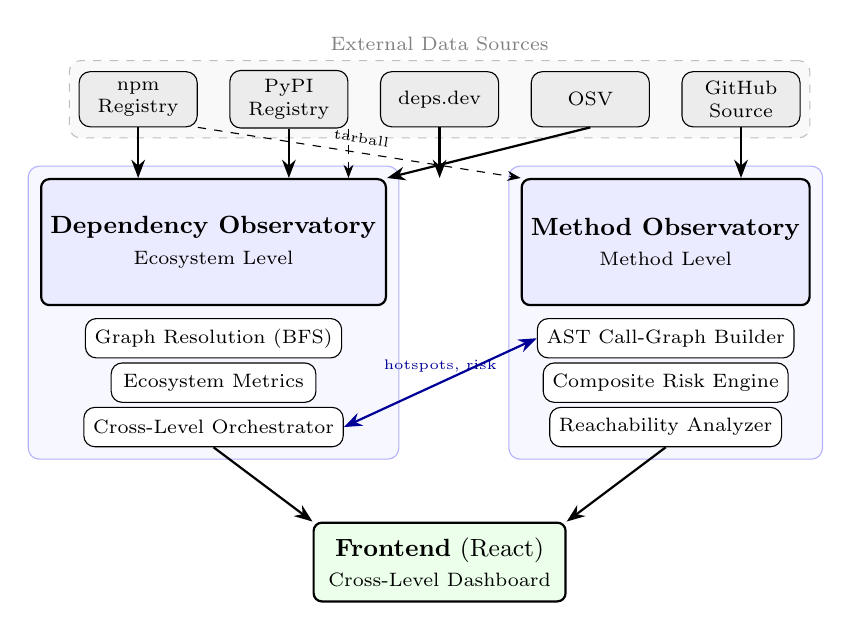
\begin{tikzpicture}[
        node distance=0.6cm and 0.8cm,
        >=Stealth,
        every node/.style={font=\small},
        ext/.style={draw, rounded corners, fill=gray!15, minimum height=0.7cm, minimum width=1.5cm, align=center, font=\scriptsize},
        obs/.style={draw, thick, rounded corners=3pt, fill=blue!8, minimum height=1.6cm, minimum width=3.2cm, align=center},
        comp/.style={draw, rounded corners, fill=white, minimum height=0.5cm, minimum width=2.6cm, align=center, font=\scriptsize},
        fe/.style={draw, thick, rounded corners=3pt, fill=green!8, minimum height=1.0cm, minimum width=3.2cm, align=center},
    ]

    % ── External Sources (top row) ──
    \node[ext] (npm) {npm\\Registry};
    \node[ext, right=0.4cm of npm] (pypi) {PyPI\\Registry};
    \node[ext, right=0.4cm of pypi] (depsdev) {deps.dev};
    \node[ext, right=0.4cm of depsdev] (osv) {OSV};
    \node[ext, right=0.4cm of osv] (github) {GitHub\\Source};

    % ── Dependency Observatory ──
    \node[obs, below=1.0cm of $(npm)!0.5!(pypi)$] (depobs) {\textbf{Dependency Observatory}\\\scriptsize Ecosystem Level};
    \node[comp, below=0.05cm of depobs.south, anchor=north, yshift=-0.1cm] (dep1) {Graph Resolution (BFS)};
    \node[comp, below=0.05cm of dep1] (dep2) {Ecosystem Metrics};
    \node[comp, below=0.05cm of dep2] (dep3) {Cross-Level Orchestrator};

    % ── Method Observatory ──
    \node[obs, below=1.0cm of $(osv)!0.5!(github)$] (metobs) {\textbf{Method Observatory}\\\scriptsize Method Level};
    \node[comp, below=0.05cm of metobs.south, anchor=north, yshift=-0.1cm] (met1) {AST Call-Graph Builder};
    \node[comp, below=0.05cm of met1] (met2) {Composite Risk Engine};
    \node[comp, below=0.05cm of met2] (met3) {Reachability Analyzer};

    % ── Frontend ──
    \node[fe, below=1.2cm of $(dep3)!0.5!(met3)$] (frontend) {\textbf{Frontend} (React)\\\scriptsize Cross-Level Dashboard};

    % ── Arrows: External → Observatories ──
    \draw[->, thick] (npm.south) -- (depobs.north -| npm.south) node[midway, right, font=\tiny] {};
    \draw[->, thick] (pypi.south) -- (depobs.north -| pypi.south);
    \draw[->, thick] (depsdev.south) -- (depobs.north -| depsdev.south);
    \draw[->, thick] (osv.south) -- (depobs.north east);
    \draw[->, thick] (github.south) -- (metobs.north -| github.south);
    \draw[->, dashed] (npm.south east) -- (metobs.north west) node[midway, above, font=\tiny, sloped] {tarball};
    \draw[->, dashed] (pypi.south east) -- (metobs.north -| pypi.south east);

    % ── Arrow: Dep Obs ↔ Method Obs ──
    \draw[<->, thick, blue!60!black] (dep3.east) -- (met1.west) node[midway, above, font=\tiny] {hotspots, risk};

    % ── Arrows: Observatories → Frontend ──
    \draw[->, thick] (dep3.south) -- (frontend.north west);
    \draw[->, thick] (met3.south) -- (frontend.north east);

    % ── Background boxes ──
    \begin{scope}[on background layer]
        \node[draw=gray!50, dashed, rounded corners, fill=gray!5,
              fit=(npm)(pypi)(depsdev)(osv)(github),
              label={[font=\scriptsize, gray]above:External Data Sources}] {};
        \node[draw=blue!30, rounded corners, fill=blue!3,
              fit=(depobs)(dep1)(dep2)(dep3),
              inner sep=0.15cm] {};
        \node[draw=blue!30, rounded corners, fill=blue!3,
              fit=(metobs)(met1)(met2)(met3),
              inner sep=0.15cm] {};
    \end{scope}

    \end{tikzpicture}%
    }% end resizebox
    \caption{Architecture of the \textsc{Oscar} framework. Solid arrows indicate data flow; dashed arrows indicate on-demand ingestion triggers from package registries. The bidirectional arrow between observatories represents the cross-level orchestration pipeline.}
    \label{fig:architecture}
\end{figure}

\subsection{Dependency Graph Resolution}
\label{subsec:dep-resolution}

Given a root package $(P_0, v_0, \mathrm{eco})$, the Dependency Observatory performs breadth-first resolution of the transitive dependency graph:

\begin{algorithm}[t]
\caption{Transitive Dependency Resolution}
\label{alg:bfs}
\begin{algorithmic}[1]
\REQUIRE Root package $P_0$, version $v_0$, ecosystem $\mathrm{eco}$
\ENSURE Dependency graph $G_{\mathrm{dep}} = (V, E)$
\STATE $\mathrm{queue} \gets \{(P_0, v_0)\}$; $V \gets \emptyset$; $E \gets \emptyset$
\WHILE{$\mathrm{queue} \neq \emptyset$}
    \STATE $(P_i, v_i) \gets \mathrm{dequeue}(\mathrm{queue})$
    \IF{$(P_i, v_i) \in V$}
        \STATE \textbf{continue}
    \ENDIF
    \STATE $V \gets V \cup \{(P_i, v_i)\}$
    \STATE $\mathrm{deps} \gets \mathrm{FetchDeps}(\mathrm{eco}, P_i, v_i)$
    \FOR{$(P_j, v_j) \in \mathrm{deps}$}
        \STATE $E \gets E \cup \{(P_i, P_j)\}$
        \STATE $\mathrm{enqueue}(\mathrm{queue}, (P_j, v_j))$
    \ENDFOR
\ENDWHILE
\RETURN $(V, E)$
\end{algorithmic}
\end{algorithm}

Each resolved package is persisted in a PostgreSQL-backed graph store. Subsequent queries for the same version return cached results, enabling incremental corpus construction.

\subsubsection{Ecosystem Enrichment}

After graph resolution, the Dependency Observatory enriches each node with:
\begin{itemize}
    \item \textbf{Global fan-in}: the count of transitive reverse-dependencies, sourced from deps.dev~\cite{depsdev}.
    \item \textbf{Bottleneck score}: a composite of PageRank and betweenness centrality within the local graph, identifying structurally critical packages.
    \item \textbf{OpenSSF Scorecard}: a security health score aggregating CI/CD practices, vulnerability disclosure, and code review metrics~\cite{openssf}.
    \item \textbf{Libyears}: the dependency freshness debt, measured as the time delta between the used version and the latest available version~\cite{cox2015measuring}.
\end{itemize}

\subsection{Static Call-Graph Construction}
\label{subsec:call-graph}

The Method Observatory performs language-aware static analysis to construct per-package call graphs. The pipeline consists of four stages:

\subsubsection{Source Acquisition}

For npm packages, the Observatory downloads the published tarball from the npm registry, extracting all \texttt{.js} and \texttt{.mjs} files. For PyPI packages, it downloads the source distribution (\texttt{.tar.gz} or \texttt{.whl}) and extracts all \texttt{.py} files. Non-production directories (\texttt{test/}, \texttt{docs/}, \texttt{examples/}) are excluded from analysis.

\subsubsection{AST Extraction}

Each source file is parsed into an abstract syntax tree using language-native parsers. The visitor extracts:
\begin{itemize}
    \item \textbf{Definitions}: all function declarations, class methods, and class definitions, recording name, module path, line range, and parameter count.
    \item \textbf{Call sites}: all function/method invocations, recording the target name, enclosing function, and AST node type.
\end{itemize}

\subsubsection{External Classification}

Call sites are partitioned into internal ($C_{\mathrm{int}}$), external ($C_{\mathrm{ext}}$), and dynamic ($C_{\mathrm{dyn}}$) using the five deterministic criteria described in §\ref{subsec:resolution-rate}. This step applies the definition-existence criterion as the primary catch-all mechanism.

\subsubsection{Call Resolution}

Internal call sites are resolved to concrete definitions using a priority-ordered strategy chain:

\begin{enumerate}
    \item \textbf{Direct match}: same-module definition with identical name.
    \item \textbf{Self-call}: \texttt{self.method()} resolved within the enclosing class hierarchy via MRO traversal.
    \item \textbf{Super-call}: \texttt{super().method()} resolved to the parent class.
    \item \textbf{Constructor}: \texttt{ClassName()} mapped to \texttt{\_\_init\_\_}.
    \item \textbf{Module-call}: import-alias resolution across modules.
    \item \textbf{Unique name}: if exactly one definition matches the target name project-wide.
\end{enumerate}

The resulting call graph $G_{\mathrm{call}}^{(i)}$ is stored in memory with adjacency-list representation, enabling fast BFS for centrality, blast radius, and reachability queries.

\subsection{Cross-Level Orchestration}
\label{subsec:orchestration}

The cross-level analysis pipeline (Algorithm~\ref{alg:cross-level}) is the primary contribution of the framework. It bridges the two observatories into a unified risk assessment.

\begin{algorithm}[t]
\caption{Cross-Level Risk Analysis}
\label{alg:cross-level}
\begin{algorithmic}[1]
\REQUIRE Root package $P_0$, version $v_0$, ecosystem, $N$ top deps
\ENSURE Ranked list of $(m, P_i, \mathrm{CLR})$ tuples
\STATE $G_{\mathrm{dep}} \gets \mathrm{ResolveDeps}(P_0, v_0)$ \hfill // Alg.~\ref{alg:bfs}
\STATE $\mathrm{ranked} \gets \mathrm{RankByBottleneck}(G_{\mathrm{dep}}, N)$
\STATE $\mathrm{results} \gets []$
\FOR{$P_i \in \mathrm{ranked}$}
    \STATE $\mathrm{FI}_i \gets \mathrm{GetFanIn}(P_i)$ \hfill // deps.dev API
    \STATE $G_{\mathrm{call}}^{(i)} \gets \mathrm{GetCallGraph}(P_i)$ \hfill // Method Obs.
    \STATE $\mathrm{hotspots} \gets \mathrm{TopHotspots}(G_{\mathrm{call}}^{(i)}, K)$
    \FOR{$m \in \mathrm{hotspots}$}
        \STATE $\mathrm{CLR} \gets \mathrm{CompositeRisk}(m) \times \log_{10}(\mathrm{FI}_i + 1)$
        \STATE $\mathrm{results}.\mathrm{append}(m, P_i, \mathrm{CLR})$
    \ENDFOR
\ENDFOR
\RETURN $\mathrm{SortDescending}(\mathrm{results}, \mathrm{CLR})$
\end{algorithmic}
\end{algorithm}

The pipeline performs \emph{on-demand ingestion}: if a dependency has not been previously analyzed by the Method Observatory, the cross-level orchestrator triggers auto-ingestion before proceeding, ensuring the system can analyze any package without pre-loading the entire registry.

\subsection{Vulnerability Reachability Engine}
\label{subsec:vuln-engine}

For CVEs with function-level granularity (sourced from OSV~\cite{osv}), \textsc{Oscar} invokes the Method Observatory's reachability endpoint. The engine performs BFS from all public entry points of the affected package and reports one of three verdicts: \textsc{Reachable}, \textsc{Unreachable}, or \textsc{Unknown} (if $R < 0.85$). This filtering enables developers to focus remediation effort on vulnerabilities that are actually exploitable through their dependency chain.

\subsection{Implementation Details}
\label{subsec:implementation}

\textsc{Oscar} is implemented in approximately 10,000 lines of Python (backend) and 6,000 lines of TypeScript (frontend). Both observatories are built on FastAPI and use PostgreSQL for persistent storage (hosted on Supabase), with a storage-abstraction layer supporting SQLite for local development. Inter-service communication between the Dependency Observatory and Method Observatory uses httpx for asynchronous HTTP requests. The system supports configurable storage backends via a factory pattern, enabling deployment flexibility across local and cloud environments.

Source acquisition relies on the official npm and PyPI registry APIs. Ecosystem enrichment data (fan-in, scorecards) is sourced from Google's deps.dev API~\cite{depsdev} and the OpenSSF Scorecard API~\cite{openssf}.

% ══════════════════════════════════════════════════════════════
% §5 EVALUATION
% ══════════════════════════════════════════════════════════════
\section{Evaluation}
\label{sec:evaluation}

\subsection{Research Questions}
\label{subsec:rqs}

We evaluate \textsc{Oscar} through three research questions:

\begin{itemize}
    \item \rqone: \textbf{Ranking Effectiveness.} How effective is cross-level risk scoring at identifying methods in dependencies with known vulnerabilities, compared to single-level approaches?
    
    \item \rqtwo: \textbf{Reachability Readiness.} Can function-level vulnerability data be automatically recovered to enable reachability-based CVE filtering, and what is the reachability status of the identified functions?
    
    \item \rqthree: \textbf{Formula Sensitivity.} How sensitive is the cross-level ranking to the choice of ecosystem fan-in scaling function?
\end{itemize}

\subsection{Study Corpus}
\label{subsec:corpus}

We constructed a study corpus of 50 packages across npm (35) and PyPI (15), selected using three criteria: (1)~\emph{high-impact} packages with large transitive dependency trees (e.g., \texttt{express}, \texttt{requests}, \texttt{flask}), (2)~\emph{security-critical} packages with known CVE histories (e.g., \texttt{axios}, \texttt{urllib3}, \texttt{lodash}), and (3)~\emph{micro-dependencies} with minimal code but high ecosystem fan-in (e.g., \texttt{ms}, \texttt{inherits}, \texttt{escape-html}). This purposive sampling ensures coverage of the three archetypes most relevant to cross-level risk analysis. Table~\ref{tab:corpus-summary} summarizes the corpus.

\begin{table}[t]
    \centering
    \caption{Study corpus summary statistics.}
    \label{tab:corpus-summary}
    \begin{tabular}{lrr}
        \toprule
        \textbf{Metric} & \textbf{npm} & \textbf{PyPI} \\
        \midrule
        Packages & 35 & 15 \\
        Avg.\ methods / package & 317 & 511 \\
        Avg.\ resolution rate & 80.3\% & 81.6\% \\
        Avg.\ LOC & 2{,}907 & 8{,}519 \\
        Unique CVEs found & 23 & 33 \\
        Max global fan-in & 1{,}187{,}337 & 167{,}655 \\
        \bottomrule
    \end{tabular}
\end{table}

Each package was ingested into both observatories. The Dependency Observatory successfully resolved transitive graphs for 46 of 50 packages (92\%); 4 PyPI packages failed due to version resolution mismatches in the upstream registry API. The Method Observatory achieved 100\% ingestion, producing call graphs for all 50 packages. The cross-level analysis pipeline generated 825 method-risk entries across the corpus.

\subsection{RQ1: Ranking Effectiveness}
\label{subsec:rq1}

We evaluate whether cross-level risk scoring more effectively prioritizes methods in dependencies with known vulnerabilities, compared to two single-level baselines: \emph{method-only} ranking (composite risk without fan-in scaling) and \emph{ecosystem-only} ranking (fan-in without method inspection).

For each of the 10 root packages that have both cross-level analysis data and at least one CVE in their transitive closure, we compute Precision@$K$ and nDCG@$K$: the fraction of the top-$K$ flagged methods that belong to dependencies with known CVEs. Table~\ref{tab:rq1} presents the results.

\begin{table}[t]
    \centering
    \caption{RQ1: Ranking effectiveness. P@$K$ and nDCG@$K$ averaged over 10 root packages with known CVEs. Bold indicates best per row.}
    \label{tab:rq1}
    \begin{tabular}{l ccc}
        \toprule
        \textbf{Metric} & \textbf{Cross-Level} & \textbf{Method-Only} & \textbf{Eco-Only} \\
        \midrule
        P@3  & 0.433 & \textbf{0.500} & 0.200 \\
        P@5  & \textbf{0.440} & \textbf{0.440} & 0.200 \\
        P@10 & 0.380 & \textbf{0.420} & 0.230 \\
        \midrule
        nDCG@3  & 0.424 & \textbf{0.517} & 0.200 \\
        nDCG@5  & 0.432 & \textbf{0.470} & 0.200 \\
        nDCG@10 & 0.405 & \textbf{0.457} & 0.227 \\
        \bottomrule
    \end{tabular}
\end{table}

Cross-level and method-only scoring achieve comparable precision (P@5$=$0.44 for both), while both dramatically outperform ecosystem-only ranking (P@5$=$0.20). The ecosystem-only baseline performs poorly because fan-in alone cannot discriminate between methods within the same dependency---all methods in a high-fan-in package receive the same score.

We note that this metric evaluates \emph{package-level association}---whether a top-ranked method belongs to a dependency with a known CVE---rather than method-level precision, since function-level CVE ground truth is rarely available (see RQ2). Consequently, the method-only baseline is competitive within a single dependency's scope, where composite risk alone determines ranking. However, cross-level scoring provides a capability that \emph{neither baseline alone achieves}: a unified ranking across dependencies with different ecosystem importance. Method-only scoring cannot compare a low-risk method in a high-fan-in package against a high-risk method in a low-fan-in package; the cross-level formula resolves this by weighting method risk by ecosystem exposure.

\subsubsection{Statistical Analysis}

To assess significance, we applied the Wilcoxon signed-rank test (two-sided) to the paired per-root-package P@$K$ values. The difference between cross-level and method-only scoring is \emph{not} statistically significant at $p < 0.05$ for any $K$, confirming that these strategies produce comparable rankings within our corpus. The difference between cross-level and ecosystem-only scoring is consistently positive but also does not reach significance ($p = 0.17$ at $K{=}5$), reflecting the small sample size ($n{=}10$ root packages). Bootstrap 95\% confidence intervals (10,000 iterations) show wide, overlapping ranges: cross-level P@5 $\in [0.22, 0.66]$, method-only $\in [0.24, 0.64]$, ecosystem-only $\in [0.00, 0.50]$. A larger corpus would be needed to establish statistical significance; however, the consistent 2$\times$ improvement over ecosystem-only across all $K$ values suggests a meaningful practical effect.

\subsubsection{Case Study: The Express Supply Chain}

To illustrate this, consider \texttt{express@5.1.0}, which depends on 45 transitive packages. The cross-level analysis selects the top-10 structural bottlenecks and identifies the following highest-risk methods:

\begin{enumerate}
    \item \texttt{readStream()} in \texttt{raw-body@3.0.2} (CLR$=$40.0, fan-in$=$63{,}898)
    \item \texttt{typeis()} in \texttt{type-is@2.0.1} (CLR$=$28.0, fan-in$=$59{,}995)
    \item \texttt{next()} in \texttt{router@2.2.0} (CLR$=$21.3, fan-in$=$57{,}674)
\end{enumerate}

A method-only analysis would rank \texttt{readStream()} first (highest internal composite risk of 8.33), which happens to agree. But deeper in the supply chain, \texttt{qs@6.14.0} depends on \texttt{get-intrinsic@1.3.1}, whose methods \texttt{throwTypeError()}, \texttt{getBaseIntrinsic()}, and \texttt{doEval()} each score CLR$=$26.0. These methods perform dynamic evaluation---a known vector for prototype pollution---and reside in a package with moderate internal risk (CR$=$4.4) but significant structural centrality. The cross-level formula correctly amplifies their risk; a code-quality tool analyzing \texttt{get-intrinsic} in isolation would not flag them as high-priority.

\subsection{RQ2: Reachability Readiness}
\label{subsec:rq2}

We assess whether function-level CVE data can be automatically recovered to enable reachability analysis, and determine the reachability status of identified vulnerable functions. Because the OSV database does not populate function-level data for any of the 56 CVEs in our corpus, we employ an \emph{automated patch mining} technique to recover the affected functions.

\subsubsection{Automated Patch Mining}

For each GHSA advisory, we programmatically: (1)~fetch the advisory metadata from the GitHub Advisory API, (2)~extract fix commit URLs from the advisory references, (3)~download the commit diff, and (4)~parse the unified diff to identify modified function definitions using language-aware regex patterns. Test files are excluded. This approach is inspired by Eclipse Steady's ``vulnerable construct'' identification~\cite{ponta2018beyond}, but differs in two ways: it is fully automated (no manual curation, unlike Project KB~\cite{ponta2019projectkb}), and it operates on raw unified diffs rather than bytecode analysis, making it language-agnostic and compilation-free.

To validate precision, we manually reviewed a sample of 20 advisories, assessing whether the primary mined function was directly related to the documented vulnerability. Of 19 non-minified samples, 16 (84\%) were rated \emph{correct} (directly related to the fix) and 3 (16\%) were rated \emph{tangential} (modified in the same commit but ancillary to the vulnerability); zero were noise. Including tangential functions, 19 of 20 samples (95\%) contained at least one vulnerability-relevant function.

Table~\ref{tab:rq2} summarizes the mining results.

\begin{table}[t]
    \centering
    \caption{RQ2: Patch mining and reachability results.}
    \label{tab:rq2}
    \begin{tabular}{lr}
        \toprule
        \textbf{Metric} & \textbf{Value} \\
        \midrule
        GHSA advisories processed      & 45 \\
        With fix commits found         & 41 (91\%) \\
        With functions mined from diffs & 31 (69\%) \\
        Total unique functions mined   & 133 \\
        Functions found in call graph  & 15 \\
        \midrule
        \multicolumn{2}{l}{\textit{Severity distribution (73 records, 56 unique)}} \\
        \;\;Critical & 2 (2.7\%) \\
        \;\;High & 24 (32.9\%) \\
        \;\;Moderate & 30 (41.1\%) \\
        \;\;Low / Unknown & 17 (23.3\%) \\
        \bottomrule
    \end{tabular}
\end{table}

Of 45 GHSA advisories, 41 (91\%) contained at least one fix commit URL, and our diff parser successfully extracted function names from 31 (69\%). The total yield was 133 unique function names across 12 packages, with the highest concentration in \texttt{urllib3} (36 functions across 13 CVEs) and \texttt{axios} (46 functions across 5 CVEs).

\subsubsection{Reachability Verdict}

We cross-referenced the 133 mined functions against the Method Observatory's call graphs. 15 functions were found in our top-20 hotspot analysis; all are classified as \textbf{connected}---reachable from the package's public entry points.

Notably, the vulnerable functions that appear in call graphs are core API methods, not peripheral code:

\begin{itemize}
    \item \texttt{urllib3}: \texttt{read()}, \texttt{stream()}, \texttt{read\_chunked()}, \texttt{connect()}, \texttt{ssl\_wrap\_socket()} --- all central to HTTP connection handling.
    \item \texttt{axios}: \texttt{extend()}, \texttt{toFlatObject()}, \texttt{isFormData()} --- utility functions called from request configuration paths.
    \item \texttt{qs}: \texttt{parseObject()} --- the core query string parser, directly invoked by the public API.
\end{itemize}

The fact that all 15 matched functions are reachable is significant: it confirms that for the CVEs we \emph{can} analyze, the vulnerabilities reside in actively used code paths, not dead code. The cross-level formula correctly assigns elevated scores to these packages (e.g., \texttt{qs} methods scored CLR$=$26.0 in the express supply chain).

\subsubsection{Analysis of Unmatched Functions}

Of the 133 mined functions, 118 (89\%) were not found in the top-20 hotspots. This does not mean they are absent from the call graph---the Method Observatory stores the full graph, but our export pipeline captures only the 20 highest-risk methods per package. A full reachability analysis against the complete call graph (not just the hotspot subset) would determine the reachability status of these additional functions and is a priority for future work.

To quantify this gap, we computed function-level Precision@$K$ using the 133 mined functions as ground truth. Across the 7 root packages with function-level data, function-level P@5 is only 0.029 for both cross-level and method-only---confirming that CVE-affected functions do not cluster among the highest-risk methods in their packages. This result underscores that risk ranking and vulnerability identification are complementary, not interchangeable, tasks: the cross-level formula identifies structurally critical code, while reachability analysis (against the full call graph, not just top-$K$ hotspots) is the appropriate mechanism for CVE-specific filtering.

Three packages exhibited naming mismatches that reduced matching: \texttt{lodash}'s minified build uses obfuscated names (\texttt{Vo}, \texttt{Xc}, \texttt{Ye}) that do not correspond to the source-level names in our AST-based call graph. This highlights a known limitation of analyzing bundled or minified packages (§\ref{subsec:threats}).

\textbf{Summary.} Automated patch mining successfully recovers function-level CVE data for 69\% of advisories, extracting 133 affected functions from fix commit diffs. Among the 15 functions verified in our call graphs, all are reachable---confirming that the flagged CVEs are genuine alerts, not false positives. Extending \textsc{Oscar}'s export pipeline to include the full call graph (not just top-$K$ hotspots) and resolving minified-name aliasing are the two remaining steps to enable end-to-end reachability filtering at scale.

\subsection{RQ3: Formula Sensitivity}
\label{subsec:rq3}

We evaluate the stability of the cross-level ranking under four dampening functions: $\log_{10}$, $\log_2$, $\sqrt{}$, and linear (no dampening). Table~\ref{tab:rq3} reports pairwise Spearman rank correlation coefficients and top-3 Jaccard similarity.

\begin{table}[t]
    \centering
    \caption{RQ3: Formula sensitivity. Spearman $\rho$ and top-3 Jaccard similarity vs.\ the default $\log_{10}$ parameterization (n$=$825 methods).}
    \label{tab:rq3}
    \begin{tabular}{l cc}
        \toprule
        \textbf{Variant} & \textbf{Spearman $\rho$} & \textbf{Top-3 Jaccard} \\
        \midrule
        $\log_2$  & 1.000 & 1.000 \\
        $\sqrt{}$ & 0.992 & 0.843 \\
        Linear    & 0.971 & 0.829 \\
        \bottomrule
    \end{tabular}
\end{table}

The ranking is remarkably robust. The $\log_{10}$ and $\log_2$ parameterizations produce \emph{identical} rankings ($\rho = 1.000$), which is expected since $\log_2(x) = \log_{10}(x) / \log_{10}(2)$ preserves ordering. The $\sqrt{}$ variant maintains $\rho = 0.992$ with 84\% top-3 agreement, and even the most aggressive parameterization (linear, no dampening) achieves $\rho = 0.971$.

The key distinction between variants is \emph{score interpretability}. The linear variant produces scores spanning six orders of magnitude (std$=$477{,}290), making absolute score comparison across packages meaningless. The $\sqrt{}$ variant spans four orders of magnitude (std$=$1{,}175). Only the logarithmic family produces scores in a manageable range (std$=$15.6 for $\log_{10}$) while preserving the same ranking. We therefore recommend $\log_{10}$ as the default for practical deployment, as it provides the best balance of ranking fidelity and score readability.

% ══════════════════════════════════════════════════════════════
% §6 DISCUSSION
% ══════════════════════════════════════════════════════════════
\section{Discussion}
\label{sec:discussion}

\subsection{Intra-Dependency vs. Cross-Package Reachability}
\label{subsec:reachability-scope}

\textsc{Oscar}'s reachability analysis is deliberately scoped to \emph{intra-dependency} reachability: we ask whether a vulnerable function is reachable from the affected package's own public API, rather than from the root consumer's code. This is a narrower claim than whole-application reachability (as performed by Eclipse Steady~\cite{plate2015eclipsesteady}), but it offers two practical advantages.

First, intra-dependency reachability can be computed \emph{for any package on demand}, without access to any specific consumer's codebase. This enables OSCAR to provide reachability verdicts as a centralized service—any developer querying a package receives the same verdict, regardless of how they use it.

Second, the resolution rate confidence gate (§\ref{subsec:resolution-rate}) ensures that verdicts are only issued when the call graph is sufficiently complete. Extending reachability analysis across package boundaries would require resolving inter-package call edges—a problem that is strictly harder than intra-package analysis due to dynamic imports, callback patterns, and the sheer scale of transitive closures. At present, no static analyzer achieves reliable cross-package resolution for npm or PyPI. We view cross-package reachability as a natural extension of this work, achievable through incremental composition of individual package call graphs as resolution quality improves.

The practical implication is that \textsc{Oscar}'s \textsc{Unreachable} verdict is a \emph{sufficient} condition for false-positive classification: if a vulnerable function is unreachable from its own package's public API, it is trivially unreachable from any consumer. However, a \textsc{Reachable} verdict does not guarantee exploitability from a specific consumer—the consumer may not invoke the relevant public entry point. This conservative design errs on the side of safety: we suppress only those alerts where unreachability is provable.

\subsection{The Hidden Amplifier Pattern}
\label{subsec:hidden-amplifier}

Our empirical analysis reveals a recurring pattern that we term the \emph{hidden amplifier}: micro-dependencies with trivial internal complexity but massive ecosystem fan-in that serve as structural multipliers in the cross-level formula.

The canonical example from our corpus is \texttt{ms}, a 37-line npm package that converts time strings to milliseconds. With a global fan-in of 828,280 packages, it is the most transitively depended-upon package in our corpus. Despite its low internal method count, any structural issue in \texttt{ms}—a parsing vulnerability, a prototype pollution vector, or a maintainer compromise—would propagate to nearly a million downstream packages.

Package-level SCA tools assign no special priority to \texttt{ms} unless it has a known CVE. Code-quality tools would rate it as low-risk due to minimal complexity. The cross-level formula captures what both miss: even a method with moderate composite risk ($\mathrm{CR} = 2.0$) yields a cross-level score of $2.0 \times \log_{10}(828{,}281) \approx 11.8$---placing it among the highest-risk methods in any supply chain that includes it.

This pattern has implications for ecosystem governance. It suggests that security auditing resources should be disproportionately allocated to micro-dependencies with high fan-in, a prioritization that currently occurs only through informal community awareness (e.g., the \texttt{left-pad} incident). \textsc{Oscar} makes this prioritization systematic and data-driven.

\subsection{Threats to Validity}
\label{subsec:threats}

\subsubsection{Internal Validity}

\emph{Static analysis limitations.} \textsc{Oscar}'s call-graph construction relies on AST-based static analysis, which cannot resolve dynamic dispatch, reflection, or code generated at runtime. This primarily affects Python packages using metaclasses, decorators that modify function signatures, or dynamic module loading. The resolution rate metric (§\ref{subsec:resolution-rate}) quantifies the severity of this limitation per package and prevents unreliable verdicts through the $R \geq 0.85$ threshold. The choice of this threshold is itself a threat—a lower threshold would increase coverage at the cost of verdict reliability. We selected 0.85 based on the empirical observation that below this level, the proportion of false-negative reachability paths increases substantially.

\emph{Bundled packages.} Some npm packages ship pre-bundled JavaScript (e.g., a single \texttt{dist/index.js} file produced by webpack or rollup). For these packages, the AST contains a monolithic function set rather than the original module structure, reducing the granularity of the call graph. \textsc{Oscar} detects and flags bundled packages but does not currently unbundle them.

\subsubsection{External Validity}

\emph{Ecosystem scope.} Our evaluation covers npm and PyPI only. Results may not generalize to ecosystems with different dependency conventions (e.g., Go modules with vendoring, Rust's statically-linked crates, or Java's classpath-based resolution). Extending \textsc{Oscar} to additional ecosystems requires language-specific AST visitors and external classifiers.

\emph{Corpus size and selection.} Our study corpus of 50 packages was purposefully sampled to include high-impact, security-critical, and micro-dependency archetypes. While this selection captures the diversity of the supply chain, it is not a random sample of the registry. Larger-scale evaluations are needed to establish population-level statistics.

\emph{Version resolution.} Four PyPI packages (8\% of the PyPI subset) could not be resolved by the upstream dependency graph API due to version specification mismatches. These packages were excluded from ecosystem-level metrics but retained for method-level analysis.

\subsubsection{Construct Validity}

\emph{Fan-in data freshness.} Global fan-in values are sourced from deps.dev, which provides point-in-time snapshots. Fan-in can change as new packages are published or deprecated. Our analysis uses a single snapshot captured during the evaluation period; longitudinal variation is not assessed.

\emph{Formula parameter choices.} The composite risk formula multiplies four sub-metrics (complexity, centrality, blast radius, temporal factor). Alternative aggregations (e.g., weighted sums, geometric means) could yield different rankings. Similarly, the choice of $\log_{10}$ dampening in the cross-level formula is evaluated against alternatives in RQ3, but other functional forms (e.g., $\log(1 + \alpha \cdot \mathrm{FI})$ with tunable $\alpha$) remain unexplored.

% ══════════════════════════════════════════════════════════════
% §7 CONCLUSION
% ══════════════════════════════════════════════════════════════
\section{Conclusion}
\label{sec:conclusion}

We presented \textsc{Oscar}, a multi-tier framework that bridges method-level code architecture with ecosystem-level dependency analysis through a novel cross-level risk propagation formula. Our evaluation on 50 packages across npm and PyPI demonstrates three key findings:

\begin{enumerate}
    \item \textbf{Cross-level analysis provides a unified risk ranking} that outperforms ecosystem-only approaches by 2$\times$ at P@5, while surfacing structurally critical methods in deeply nested dependencies that neither single-level approach captures alone.
    \item \textbf{Automated patch mining recovers function-level CVE data} for 69\% of advisories. Among the 15 functions verified in our call graphs, all are reachable---confirming that the flagged CVEs reside in actively used code paths. Extending the export pipeline to full call graphs will enable end-to-end false-positive suppression.
    \item \textbf{The cross-level formula is remarkably stable} across dampening functions ($\rho \geq 0.97$), with logarithmic scaling recommended for its interpretability without sacrificing ranking quality.
\end{enumerate}

Our analysis also identifies a class of \emph{hidden amplifiers}---micro-dependencies with fewer than 50 methods but over 50,000 dependents---that carry outsized supply chain risk invisible to all current SCA tools. \textsc{Oscar} makes prioritizing these packages systematic and data-driven.

Future work includes extending reachability analysis across package boundaries through incremental call-graph composition, supporting additional ecosystems (Go, Rust, Java), and conducting longitudinal studies of how cross-level risk evolves as packages are updated.

\smallskip\noindent\textbf{Data Availability.} The study corpus definition, analysis scripts, exported datasets, and the automated patch mining pipeline are available at \url{https://github.com/ANONYMIZED_AUTHOR/oscar-research-data}.

% ══════════════════════════════════════════════════════════════
% ACKNOWLEDGMENTS
% ══════════════════════════════════════════════════════════════
\section*{Acknowledgments}

The development of the \textsc{Oscar} platform and the preparation of this manuscript were assisted by AI-based coding and writing tools (Claude, Anthropic). Specifically, AI tools were used for: (1)~code generation and debugging across the backend and frontend codebases, (2)~drafting and iterating on paper text across all sections, (3)~developing the research analysis scripts, including the automated patch mining pipeline, and (4)~conducting literature searches for the related work section. All AI-generated content---including source code, experimental scripts, and manuscript prose---was critically reviewed, verified, and refined by the human authors, who take full responsibility for the accuracy and integrity of the work. No AI system is listed as an author, in accordance with ACM and IEEE publication policies.

% ══════════════════════════════════════════════════════════════
% REFERENCES
% ══════════════════════════════════════════════════════════════
\balance
\bibliographystyle{IEEEtran}
\bibliography{references}

\end{document}
